\documentclass[tikz,border=8pt]{standalone}
% Shared look for every TikZ diagram. Load with \input{../../tools/tikz-style.tex}
\usepackage[T1]{fontenc}
\usepackage{lmodern}
\renewcommand{\sfdefault}{lmr}  % diagrams use the same serif as the text
\usetikzlibrary{arrows.meta, positioning, shapes.geometric, calc, fit, backgrounds}
\definecolor{cblue}{HTML}{4C78A8}
\definecolor{corange}{HTML}{F58518}
\definecolor{cgreen}{HTML}{54A24B}
\definecolor{cred}{HTML}{E45756}
\definecolor{cpurple}{HTML}{B279A2}
\definecolor{cgrey}{HTML}{6B6B6B}
\tikzset{
  every picture/.style={font=\sffamily, line width=1.2pt},
  box/.style={draw=#1, fill=#1!12, rounded corners=4pt, align=center, inner sep=7pt, minimum height=1.1cm},
  box/.default=cgrey,
  arrow/.style={-{Stealth[length=3mm]}, draw=cgrey, line width=1.4pt},
  title/.style={font=\sffamily\bfseries\Large},
  note/.style={font=\sffamily\small, text=cgrey, align=center},
}
\AtBeginDocument{\hyphenpenalty=10000 \exhyphenpenalty=10000}

\begin{document}
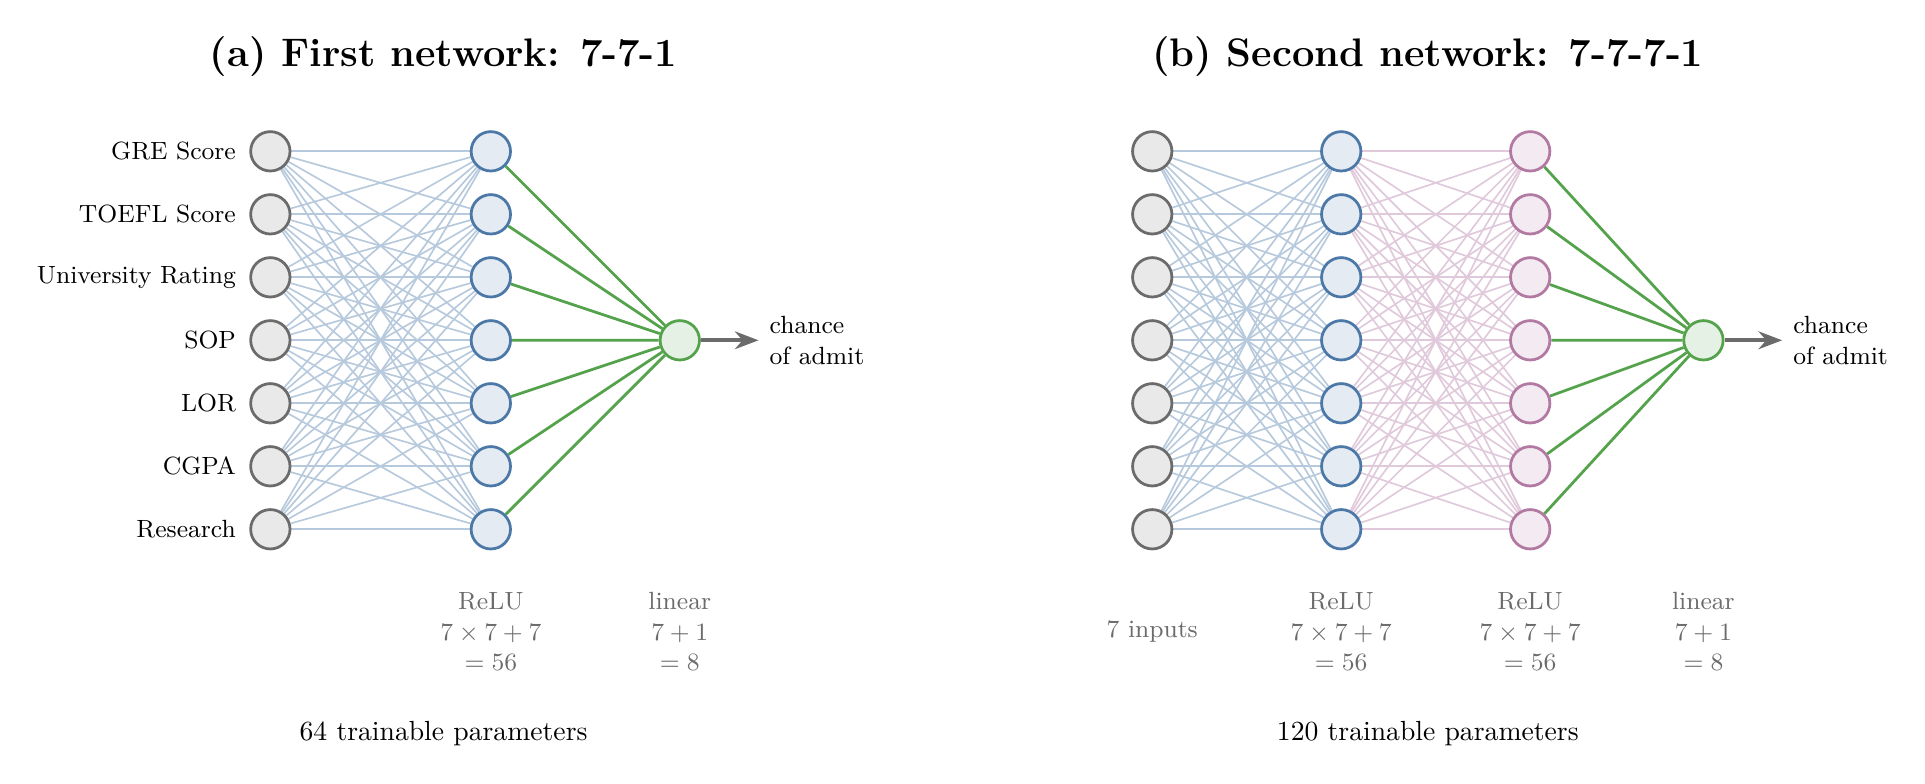
\begin{tikzpicture}[
  inp/.style={circle, draw=cgrey, fill=cgrey!15, minimum size=0.5cm, inner sep=0pt, line width=1pt},
  hid/.style={circle, draw=#1, fill=#1!15, minimum size=0.5cm, inner sep=0pt, line width=1pt},
  lab/.style={font=\sffamily\small, anchor=east}]
  % ---------- (a) first network: 7-7-1 ----------
  \foreach \n [count=\i] in {GRE Score, TOEFL Score, University Rating, SOP, LOR, CGPA, Research} {
    \node[inp] (a0\i) at (0, -0.8*\i) {};
    \node[lab] at (-0.3, -0.8*\i) {\n};
    \node[hid=cblue] (a1\i) at (2.8, -0.8*\i) {};
  }
  \node[hid=cgreen] (a2) at (5.2, -3.2) {};
  \begin{scope}[on background layer]
    \foreach \i in {1,...,7} \foreach \j in {1,...,7} \draw[cblue!40, line width=0.6pt] (a0\i) -- (a1\j);
    \foreach \j in {1,...,7} \draw[cgreen, line width=1pt] (a1\j) -- (a2);
  \end{scope}
  \draw[arrow] (a2) -- ++(1.0,0) node[right, align=left, font=\sffamily\small] {chance\\of admit};
  \node[title] at (2.2, 0.4) {(a) First network: 7-7-1};
  \node[note] at (2.8, -6.9) {ReLU\\$7 \times 7 + 7$\\$= 56$};
  \node[note] at (5.2, -6.9) {linear\\$7 + 1$\\$= 8$};
  \node[font=\sffamily\normalsize] at (2.2, -8.2) {64 trainable parameters};
  % ---------- (b) second network: 7-7-7-1 ----------
  \begin{scope}[xshift=11.2cm]
    \foreach \i in {1,...,7} {
      \node[inp] (b0\i) at (0, -0.8*\i) {};
      \node[hid=cblue] (b1\i) at (2.4, -0.8*\i) {};
      \node[hid=cpurple] (b2\i) at (4.8, -0.8*\i) {};
    }
    \node[hid=cgreen] (b3) at (7.0, -3.2) {};
    \begin{scope}[on background layer]
      \foreach \i in {1,...,7} \foreach \j in {1,...,7} {
        \draw[cblue!40, line width=0.6pt] (b0\i) -- (b1\j);
        \draw[cpurple!40, line width=0.6pt] (b1\i) -- (b2\j);
      }
      \foreach \i in {1,...,7} \draw[cgreen, line width=1pt] (b2\i) -- (b3);
    \end{scope}
    \draw[arrow] (b3) -- ++(1.0,0) node[right, align=left, font=\sffamily\small] {chance\\of admit};
    \node[title] at (3.5, 0.4) {(b) Second network: 7-7-7-1};
    \node[note] at (0, -6.9) {7 inputs};
    \node[note] at (2.4, -6.9) {ReLU\\$7 \times 7 + 7$\\$= 56$};
    \node[note] at (4.8, -6.9) {ReLU\\$7 \times 7 + 7$\\$= 56$};
    \node[note] at (7.0, -6.9) {linear\\$7 + 1$\\$= 8$};
    \node[font=\sffamily\normalsize] at (3.5, -8.2) {120 trainable parameters};
  \end{scope}
\end{tikzpicture}
\end{document}
